\newpage
\section{Processamento de sinais}


O projeto da equipe de processamento de sinais consiste no recebimento dos dados enviados pela placa \textit{NI 6320}, processamentos dos valores fornecidos e, por meio de uma interface gráfica de controle, dar ao operador a decisão de qual o comportamento o sistema deve tomar.

\subsection{Levantamento dos materiais}

É possível fazer a mesma operação de processamento de sinais com placas como:
\begin{itemize}
    \item Arduino
    \item Raspberry Pi
    \item NI 6320
    
\end{itemize}

A escolha da placa NI 6320, se da pelas facilitações para sistemas de arrefecimento, descritas em seu manual. Estas placas são indicadas para aplicações de controle a automação de medição. O que justifica a funcionalidade desejada no projeto a ser desenvolvido.


Abaixo segue uma tabela descritiva de tal placa.

    \begin{table}[htb]
        \centering
        \begin{tabular}{|p{3cm}|p{3cm}|}
        \hline
        NI 6320  & \\ \hline
        Preço(R\$) & R\$ 2,470.00 \\ \hline
        Cliente já possui? & Possui \\ \hline
        Implementação da solução & Software de apoio e fornecimento dos dados já implementados\\ \hline
        \end{tabular}
        \caption{Detalhamento da placa NI 6320}
        \end{table}


Devido ao cliente já possuir um exemplar para uso e a placa possuir muitas facilidades para o tipo de projeto que será desenvolvido por possuir um conversor analógico-digital com uma boa resolução (12 bits/Sample) e uma taxa de amostragem de 250kS/s, a placa \textit{NI 6320} apresenta melhores opções para o projeto.
A placa \textit{NI 6320} também pode ser utilizada com o software \textit{LabView}, o qual será utilizado para implementação do software ,que facilita na implementação de soluções com as características presentes no projeto.

\subsection{Construção do Software}

A construção do Software responsável pelo processamento de sinais foi feito utilizando o programa LabVIEW que é um software de engenharia de sistemas criado especificamente para aplicações que envolvam teste, medição e controle, com rápido acesso ao hardware e a informações obtidas a partir dos dados.
A construção de sistemas utilizando o LabVIEW é feita utilizando blocos, onde cada bloco desempenha uma função específica e se relaciona com outros blocos de acordo com a construção do diagrama.
Segue abaixo o diagrama que será utilizado na placa já especificada para fazer o processamento de sinais e garantir que o sistema terá o comportamento correto. Para melhor compreensão do diagrama, ele será descrito por partes.

\subsubsection{Temperatura}

\begin{figure}[!htb]                                                             
    \centering                                                                      
    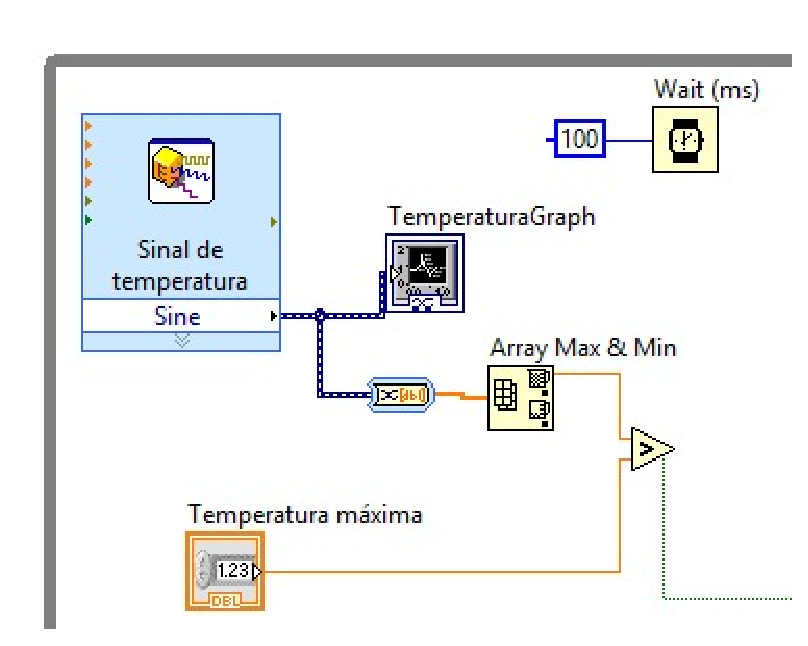
\includegraphics[scale=0.6, keepaspectratio=true]{figuras/detalhado/temp_labview.eps} 
    \caption{Diagrama de blocos da parte de temperatura}\label{temp1}
 \end{figure}

 Na figura \ref{temp1}, o primeiro bloco, Sinal de temperatura é responsável por simular a entrada de temperatura, que será coletada e fornecida pelo sistema elaborado pelo equipe de controle, o bloco seguinte é o TemperaturaGraph, ele mostra os resultados coletados na tela de controle do sistema. A seguir existe o bloco do Conversor, que manda um valor do tipo double para o bloco seguinte. Por fim, o bloco Array max \& Min pega o valor máximo e mínimo do array recebido, pois para o sistema em questão só é relevante o valor máximo para ser comparado com o valor máximo aceitável em relação à temperatura.
O bloco com um “relógio” é um delay aplicado de 100(ms). Por fim, o bloco Temperatura máxima insere o valor máximo, digitado pelo usuário, aceitável pelo sistema para ser verificado no bloco de comparação.

\subsubsection{Fluxo}


\begin{figure}[!htb]                                                               
    \centering                                                                      
    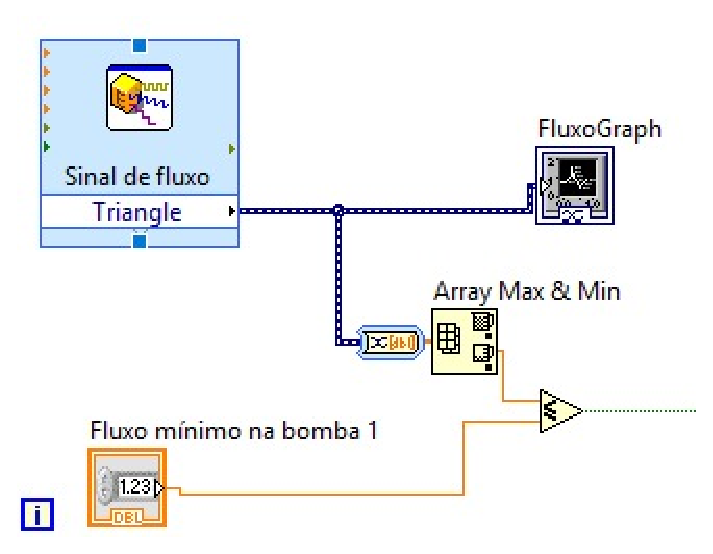
\includegraphics[scale=0.6, keepaspectratio=true]{figuras/detalhado/flux.eps} 
    \caption{Diagrama de blocos da parte de fluxo}
 \end{figure}

O bloco inicial desta parte do diagrama é o Sinal de fluxo, ele vai gerar os valores que simulam o fluxo de água coletados pelo time de controle. Em seguida existe o bloco FluxoGraph, que mostra os resultados coletados no painel que interage com o usuário.
    Assim como no tópico anterior, existe um Conversor que transforma os valores coletados para o tipo double. O bloco  Array Max \& Min pega o maior valor do array repassado pelo bloco anterior e compara com o valor mínimo aceitável.
    A comparação por fim é feita com o Fluxo mínimo na bomba 1 com os blocos descritos acima, caso o valor seja inferior ou igual o valor informado pelo usuário o sistema liga uma bomba secundária para garantir que o sistema não terá problemas.

\subsubsection{Dispositivos}

\begin{figure}[!htb]                                                               
    \centering                                                                      
    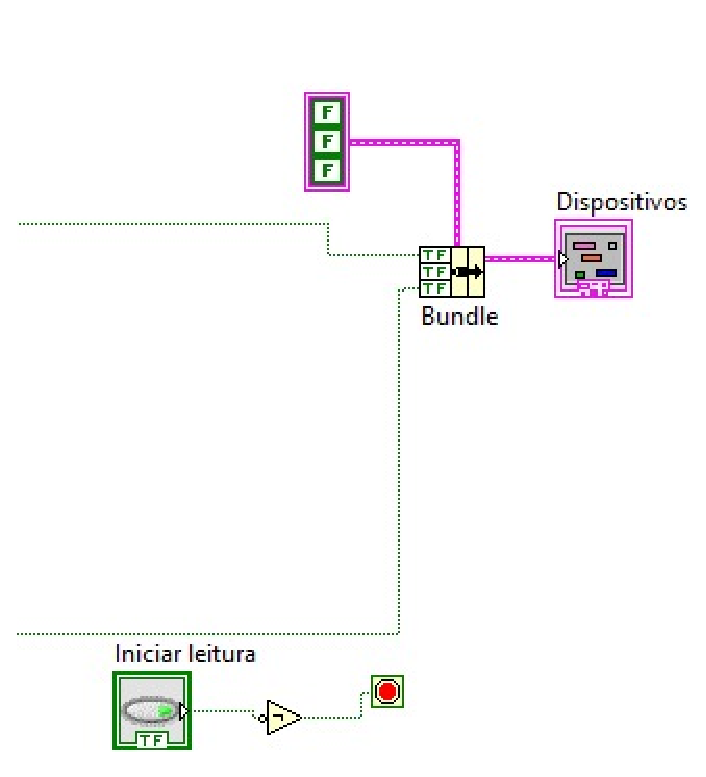
\includegraphics[scale=0.6, keepaspectratio=true]{figuras/detalhado/_bundle.eps} 
    \caption{Diagrama de blocos de dispositivos}
 \end{figure}

O bloco Iniciar leitura, é responsável pela interação com o usuário para que seja possível iniciar e pausar o sistema. As três letras F representam valores booleanos que também fazem parte da interação com o usuário.
    Bundle e Dispositivos são os blocos finais que servem para interação com a interface de usuário.

\newpage
\subsubsection{Diagrama de blocos completo}
\begin{figure}[!htb]\label{completo}                                                         
    \centering                                                                      
    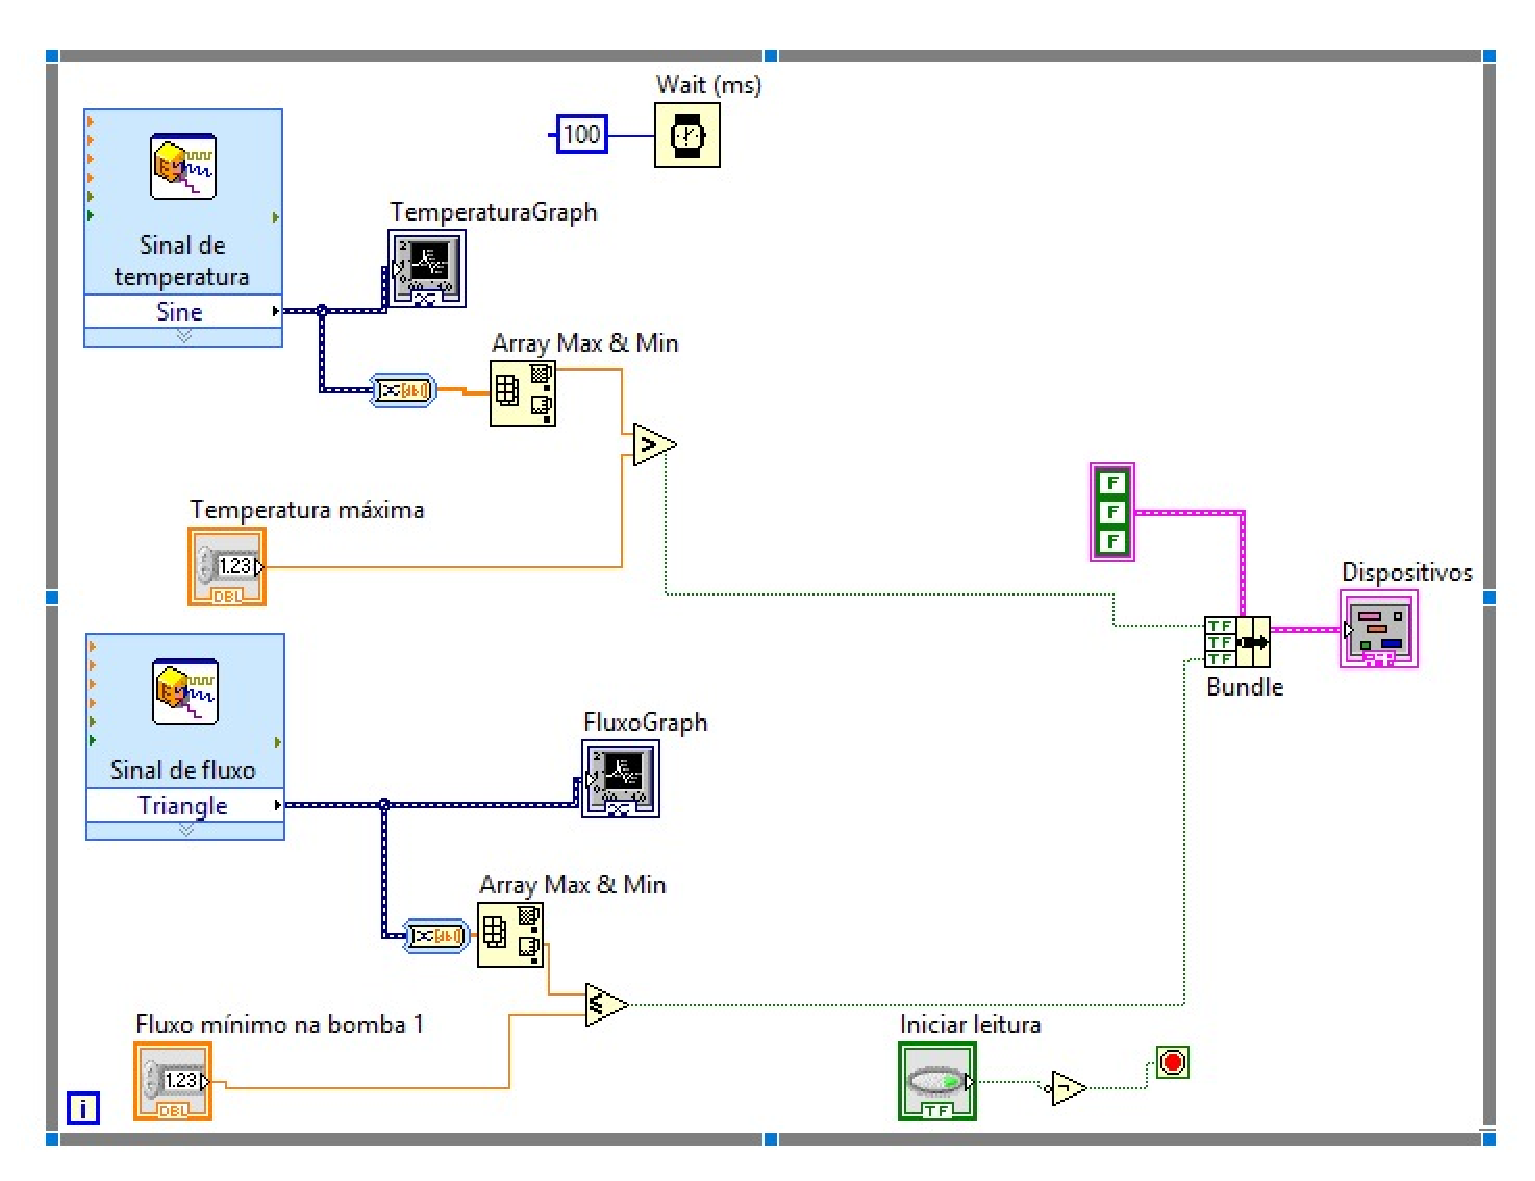
\includegraphics[scale=0.4, keepaspectratio=true]{figuras/detalhado/completo.eps} 
    \caption{Diagrama de funcionamento completo}\label{dcompl}
 \end{figure}

Após descrever cada parte do diagrama, é possivel observar o diagrama completo na figura \ref{dcompl}.


\subsubsection{Interface de usuário criada no LabView}

A imagem abaixo representa a tela que será apresentada ao usuário de forma que se possa utilizar o software.

\begin{figure}[!htb]                                                               
    \centering                                                                      
    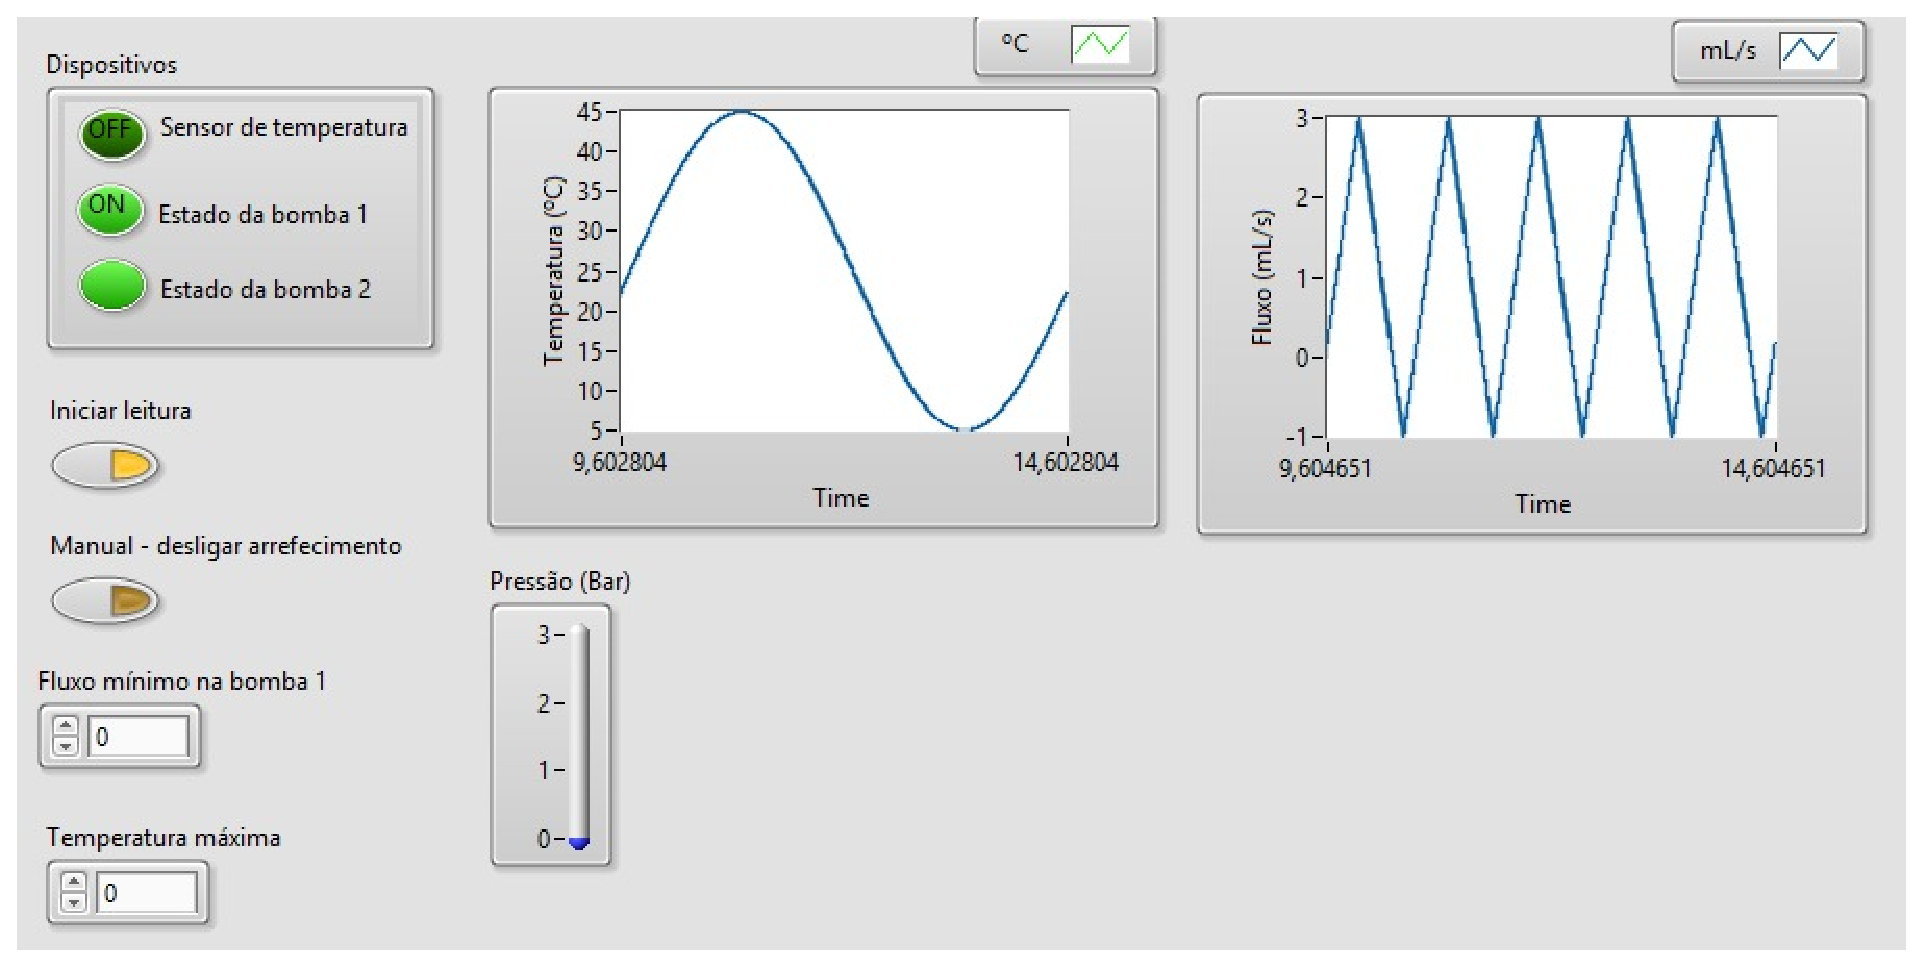
\includegraphics[scale=0.4, keepaspectratio=true]{figuras/detalhado/userinterface.eps} 
    \caption{Interface de usuário}
 \end{figure}